\documentclass[10pt]{exam}
\usepackage[hon]{template-for-exam}
\usepackage{fancybox,tikz}
\usetikzlibrary{shadings,decorations.pathmorphing,arrows.meta,patterns}

\title{Vector Addition with Vector Components}
\author{Rohrbach}
\date{\today}

\begin{document}
\maketitle


\begin{questions}

\question
  An airplane is taking off at a 57° angle with a velocity of 45 m/s.  How fast is it traveling across the ground, as well as into the air?
  \vs
  
\question
  Sandy Squirrel travels 18 m east and 41 m north to get to her secret stash of Emerald Nuts.  Chester Chipmunk decides to take a short cut and travel in a straight line to the location of the (not so) secret stash.  How far did he travel and at what angle?
  \vs

\question
  Draw each of the following vectors and calculate the $x$- and $y$- components.
  %
  \begin{align*}
    \vec{A} &= \SI{9}{m}  \text{ @ 35$^\circ$ N of E} &
    \vec{B} &= \SI{12}{m}  \text{ @ 70$^\circ$ E of S} &
    \vec{C} &= \SI{25}{m} \text{ @ 12$^\circ$ W of S} 
  \end{align*}

  \vs[2]


\pagebreak

\begin{Sbox}\begin{minipage}{6.3in}

  \section*{Vector Addition}

  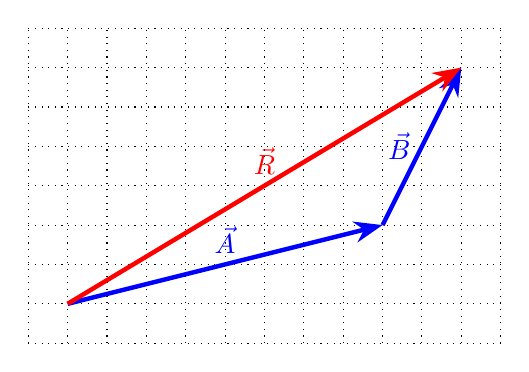
\begin{tikzpicture}
    %\draw[gray,dashed,thin] (0,0) grid (16,10);
    \draw[dotted,thin] (0,0) grid[step=0.5] (6,4);
    \begin{scope}[ultra thick,-Stealth]
      \draw[blue] (0.5,0.5) coordinate (O) -- ++(4,1) 
        coordinate (A) node[midway,above] {$\vec{A}$};
      \draw[blue] (A) -- ++ (1,2) 
        coordinate (B) node[midway,left] {$\vec{B}$};
      \draw[red] (O) -- (B) node[midway,above] {$\vec{R}$};
    \end{scope}
  \end{tikzpicture} 

\end{minipage}\end{Sbox}

\noindent
\uplevel{\shadowbox{\TheSbox}}


\question

  Consider the following vectors:
  %
  \begin{align*}
    \vec{D} &= \SI{30}{m} \text{ @ 60$^\circ$ N of W} \\
    \vec{E} &= \SI{5}{m} \text{, \sc East}
  \end{align*}
  %
  Calculate $\vec{R}=\vec{A}+\vec{B}$.

  \vs[3]
  
\end{questions}

\end{document}